%%%%%%%%%%%%%%%%%%%%%%%%%%%%%%%%%%%%%%%%%%%%%%%%%%%%%%%%%%%%%%%%%%%%%
% Template for Master work
%%%%%%%%%%%%%%%%%%%%%%%%%%%%%%%%%%%%%%%%%%%%%%%%%%%%%%%%%%%%%%%%%%%%%%
\documentclass[12pt,a4paper,notitlepage,colorinlistoftodos]{article} 
% can add 'draft' to unload figures

% Quick set up
\usepackage{ifthen} \newboolean{notes} \newboolean{terminal} \newboolean{counter}
\setboolean{notes}{true} \setboolean{terminal}{true}  \setboolean{counter}{true}
% terminal set a dark document and enable the word counter, notes put to do notes.
\newboolean{bib_basic} \setboolean{bib_basic}{true}
% bib_basic use authordate format, while when false you can provide a .bst file (change in line :
\newboolean{redef_title} \setboolean{redef_title}{false} 
\newboolean{page_title} \setboolean{page_title}{true}
% true+both minimal first page
% false+true beautiful first page
% false+false no title page
\newboolean{title_follow}
\ifthenelse{\boolean{redef_title}}{
	\setboolean{title_follow}{true}
}{
	\ifthenelse{\boolean{page_title}}{
		\setboolean{title_follow}{true}
	}{
		\setboolean{title_follow}{false}
	}
} % Globally set up abstract, list of content in newpages or not depending on the title page format.
%%%%%%%%%%%%%%%%%%%%%%%%%%%%%%%%%%%%%%%%%%%%%%%%%%%%%%%%%%%%%%%%%%%%%
%===================================================================%
%\begin{} Hiding most package loading and precisions
%===================================================================%
% Encoding and Language
\usepackage[utf8]{inputenc} % encoding
\usepackage[T1]{fontenc}

\usepackage{mathptmx} % Police Times si compilateur pdfLatex
\usepackage{parskip} % to allow multilines equations
\usepackage{amsmath}

% language
\usepackage[french]{babel} % or 'english'
% Don't forget to change the table of content
% add '\-' to create custom hypernation if a word is difficult to cut or :
\hyphenation{geo-graphique} % exemple
%% texmaker change language for auto correction
%%fr folder : /usr/share/myspell/dicts/fr_FR.dic
%%uk folder : /usr/share/hunspell/en_GB.dic

%%%%%%%%%%%%%%%%%%%%%%%%%%%%%%%%%%%%%%%%%%%%%%%%%%%%%%%%%%%%%%%%%%%%%
% Page Style
\usepackage{geometry}
%\geometry{a4paper} % format de feuille
\geometry{top=2.5cm, bottom=2.5cm, left=2.5cm, right=2.5cm} %marges
\linespread{1.5} % interligne
\usepackage{fancyhdr} %en tete et pied de page
\usepackage{lastpage}  %marche pas chez julia
\pagestyle{plain} 

% possibility to modulate the pagestyle : 
%\pagestyle{fancy}
%\chead{\includegraphics[width=\linewidth]{head.png}}
%\setlength\headheight{2.5cm}
%\lhead{}
%\rhead{}
%\cfoot{\thepage} % get rid of the page number
%\renewcommand{\headrulewidth}{0pt}
%\renewcommand{\footrulewidth}{1pt}

% specific packages :
\usepackage{lscape} % use : \begin{landscape} ... \end{landscape}
\usepackage{multicol} % use : \begin{multicols}{2} ... \end{multicols}
\setlength{\columnsep}{1cm}
\usepackage{lipsum} % use : \lipsum[1-3]

% Skip an all paragraphe use : \iffalse ... \fi

%%%%%%%%%%%%%%%%%%%%%%%%%%%%%%%%%%%%%%%%%%%%%%%%%%%%%%%%%%%%%%%%%%%%%
% Figures
\usepackage{wrapfig} 
\usepackage{graphicx, subcaption, setspace, booktabs, wrapfig}
\graphicspath{{fig/}{../fig/}}

% New captions
\usepackage{caption}
\DeclareCaptionType{annexe}[Annexe][Liste d'annexes] % Add Annexes
\DeclareCaptionType{web}[Web][Sites Web] % Add captions web

% Colours
\usepackage[table,dvipsnames*,svgnames]{xcolor} % allow to put colour in table and correct a bug in names
% option 'gray' emulate a gray scale print of the document
\definecolor{babyblue}{rgb}{0.54, 0.81, 0.94} % define new colours %http://latexcolor.com/ 
\definecolor{bleudefrance}{rgb}{0.19, 0.55, 0.91}
\definecolor{saffron}{rgb}{0.96, 0.77, 0.19}

% Highlight
\usepackage{soul}
\newcommand{\hlc}[2][yellow]{ {\sethlcolor{#1} \hl{#2}} }

% Notes and Terminal view
\ifthenelse{\boolean{terminal}}{
	\usepackage{pagecolor} % change the page color
	\pagecolor{darkgray} \color{lightgray}
	\sethlcolor{bleudefrance} % colour to highlight in terminal mod
	\ifthenelse{\boolean{notes}}{
		\usepackage[backgroundcolor=black]{todonotes} 
	}{
		\usepackage[disable]{todonotes}
	}
}{
	\sethlcolor{yellow} % colour to highlight
	\ifthenelse{\boolean{notes}}{
		\usepackage[backgroundcolor=orange]{todonotes} 
	}{
		\usepackage[disable]{todonotes}
	}
}

%%%%%%%%%%%%%%%%%%%%%%%%%%%%%%%%%%%%%%%%%%%%%%%%%%%%%%%%%%%%%%%%%%%%%
% Boxes
\usepackage[export]{adjustbox}
\newenvironment{wordbox}{% % a box with a title 'Glossary'
    \noindent
    %\refstepcounter{bluebox}
    \color{black}
    \adjustbox{innerenv={varwidth}{\dimexpr\linewidth-2\fboxsep-0.45cm\relax},
    margin=\fboxsep+.25cm \fboxsep+.2cm,bgcolor=saffron,frame,center}\bgroup  
    \textbf{Glossary}
}{%
    \egroup
}

\newcounter{bluebox}[section]
\newenvironment{bluebox}[1]{% % a boxe with a caption and number
    \noindent
    \refstepcounter{bluebox}
    \color{black}
    \adjustbox{innerenv={varwidth}{\dimexpr\linewidth-2\fboxsep-0.45cm\relax},
    margin=\fboxsep+.25cm \fboxsep+.2cm,bgcolor=saffron,frame,center}\bgroup  
    \textbf{Boxe~\thebluebox : #1}
}{%
    \egroup
}

%%%%%%%%%%%%%%%%%%%%%%%%%% Code R   %%%%%%%%%%%%%%%%%%%%%%%%%%%%%%%%%%%%%%
\usepackage{listings}
%http://latexcolor.com/ 
\definecolor{codegray}{rgb}{0.5,0.5,0.5}
\definecolor{cerulean}{rgb}{0.0, 0.48, 0.65}
\definecolor{beaublue}{rgb}{0.95, 0.95, 0.95}
\definecolor{amber}{rgb}{1.0, 0.25, 0.0}
\definecolor{indiagreen}{rgb}{0.07, 0.53, 0.03}
\definecolor{number}{rgb}{0.01, 0.01, 0.01}

\lstset{language = R,
    basicstyle=\footnotesize\color{black},
    breaklines=true,
    keepspaces=true,
    firstnumber=1,
    numbers=left, % where line-numbers; possible values (none, left, right)
    numbersep=5pt,  % how far the line-numbers are from the code
    numberstyle=\color{number},
    deletekeywords={_,/,C,troll,approx,min},
    backgroundcolor=\color{beaublue},   
    commentstyle=\color{indiagreen},
    keywordstyle=\color{amber},
    stringstyle=\color{cerulean}
    }
    
%\begin{lstlisting}
%  %%%% put the R code here %%%%
%\end{lstlisting}

%%%%%%%%%%%%%%%%%%%%%%%%%% LATEX DIFF %%%%%%%%%%%%%%%%%%%%%%%%%%%%%%%%%%%%%%%%%%%
% use terminal: latexdiff ancientfile.tex newfile.tex > revisionfile.tex

%DIF UNDERLINE PREAMBLE %DIF PREAMBLE
\RequirePackage[normalem]{ulem} %DIF PREAMBLE
\RequirePackage{color}\definecolor{RED}{rgb}{1,0,0}\definecolor{BLUE}{rgb}{0,0,1} %DIF     PREAMBLE
\providecommand{\DIFadd}[1]{{\protect\color{blue}\uwave{#1}}} %DIF PREAMBLE
\providecommand{\DIFdel}[1]{{\protect\color{red}\sout{#1}}}                      %DIF PREAMBLE
%DIF SAFE PREAMBLE %DIF PREAMBLE
\providecommand{\DIFaddbegin}{} %DIF PREAMBLE
\providecommand{\DIFaddend}{} %DIF PREAMBLE
\providecommand{\DIFdelbegin}{} %DIF PREAMBLE
\providecommand{\DIFdelend}{} %DIF PREAMBLE
%DIF FLOATSAFE PREAMBLE %DIF PREAMBLE
\providecommand{\DIFaddFL}[1]{\DIFadd{#1}} %DIF PREAMBLE
\providecommand{\DIFdelFL}[1]{\DIFdel{#1}} %DIF PREAMBLE
\providecommand{\DIFaddbeginFL}{} %DIF PREAMBLE
\providecommand{\DIFaddendFL}{} %DIF PREAMBLE
\providecommand{\DIFdelbeginFL}{} %DIF PREAMBLE
\providecommand{\DIFdelendFL}{} %DIF PREAMBLE
%DIF END PREAMBLE EXTENSION ADDED BY LATEXDIFF

%%%%%%%%%%%%%%%%%%%%%%%%%%%%%%%%%%%%%%%%%%%%%%%%%%%%%%%%%%%%%%%%%%%%%
% Word count
\usepackage{moreverb} % for verbatim ouput
\usepackage{alltt}
% Count of words
\immediate\write18{texcount -inc -incbib 
-sum Master_report.tex > /tmp/wordcount.tex}
\newcommand\wordcount{
\begin{alltt}
\input{/tmp/wordcount.tex}
\end{alltt}
}

%%%%%%%%%%%%%%%%%%%%%%%%%%%%%%%%%%%%%%%%%%%%%%%%%%%%%%%%%%%%%%%%%%%%%
% References
\usepackage{hyperref,url} % lien cliquables
\hypersetup{
colorlinks = true,
linkcolor = black,
citecolor = black,
urlcolor = black
} % https://tex.stackexchange.com/questions/50747/options-for-appearance-of-links-in-hyperref

%%%%%%%%%%%%%%%%%%%%%%%%%%%%%%%%%%%%%%%%%%%%%%%%%%%%%%%%%%%%%%%%%%%%%
% Bibliography style
\ifthenelse{\boolean{bib_basic}}{
	\usepackage[square,sort,comma,numbers]{natbib}
	\setcitestyle{authoryear,open={(},close={)}}
	\renewcommand{\bibsection}{}
}{
	\usepackage[numbers]{natbib}
}

\usepackage{chapterbib}

%%%%%%%%%%%%%%%%%%%%%%%%%%%%%%%%%%%%%%%%%%%%%%%%%%%%%%%%%%%%%%%%%%%%%
% Custom document commands
\renewcommand*\contentsname{Table des matières}
%\newcommand{\defi}[2]{\textbf{#1: }{#2}}
\newcommand{\defi}[2]{\textbf{#1: }{#2}}
\newcommand{\imp}[1][this!]{ {\todo[inline,color=red]{\textbf{Check: #1}} } }

%%%%%%%%%%%%%%%%%%%%%%%%%%%%%%%%%%%%%%%%%%%%%%%%%%%%%%%%%%%%%%%%%%%%%%
% Stuff I don't know :
\iffalse
\usepackage{gensymb}
\usepackage{xkeyval}
\usepackage{tikz}
\usepackage[para,online,flushleft]{threeparttable}
\usepackage{longtable}
\fi
%===================================================================%
%\end{}
%===================================================================%
%%%%%%%%%%%%%%%%%%%%%%%%%%%%%%%%%%%%%%%%%%%%%%%%%%%%%%%%%%%%%%%%%%%%%%
% Page de garde
%===================================================================%
%\begin{} Hiding title page 
%===================================================================%
%%%%%%%%%%%%%%%%%%%%%%%%%%%%%%%%%%%%%%%%%%%%%%%%%%%%%%%%%%%%%%%%%%%%%%
% Informations :
\title{\textbf{Title which is really important and not so much clickbait}}
\author{Maxime Jaunatre $^1$ , Master 2 BEE Grenoble}
\date{\today~|  Soutenance : mardi X décembre 2019 }

\ifthenelse{\boolean{redef_title}}{
%redefine make title
\makeatletter
    \def\@maketitle{%
  \newpage
  %\null
  %\vskip 1em%
  %\begin{center}%
  %\includegraphics[width=\textwidth]{main_head.png}
  %\end{center}%
  \let \footnote \thanks
    {\LARGE \noindent \@title  \par }%
     \vskip .5em
     \noindent  \textit{\@date} \\
    \large \noindent  \@author \\
    \footnotesize \noindent  \href{mailto:maxime.jaunatre@etu.univ-grenoble-alpes.fr}{Mail}
   
   % {\large
      %\lineskip .5em%
    %  \begin{tabular}[t]{l}%
    %   \noindent  \@author \\
     %  \noindent  \href{mailto:maxime.jaunatre@etu.univ-grenoble-alpes.fr}{Mail $^1$}
     % \end{tabular}\par}%
    %\vskip 1em%
    %{\large \@date}%

  %\par
  %\vskip .5em
  }
\makeatother
}{}

% loading subfiles that can compile on their own
\usepackage{subfiles}
\providecommand{\main}{.}  % *Modification: define file location
\def\biblio{
	\newpage
	\subsection*{Bibliographie}
	\imp[change bibliography model]
	\ifthenelse{\boolean{bib_basic}}{
		\bibliographystyle{authordate1}
	}{
		\bibliographystyle{tree}
		%\bibliographystyle{mee}
	}
	%\bibliographystyle{authordate1}
	\bibliography{\main/ICU}
}

\def\sub_title{
\begin{figure}
   \centering
    \begin{minipage}{.75\textwidth}
    \begin{center}
    {\Large Title which is really important and not so much clickbait}
    \end{center}
    %\vspace{\baselineskip}
    %\setlength{\parskip}{\smallskipamount}
    \rule{7em}{.4pt}\par
    %\todo[color = red]{put ellie}
     Maxime Jaunatre $^1$ ~ | Master 2 BEE Grenoble \par 
	\href{mailto:maxime.jaunatre@etu.univ-grenoble-alpes.fr}{Mail $^1$}~| \today \par 
    \textbf{This is a subfile from the Master\_report.tex file}
\end{minipage}
\end{figure}
\hrule
}
%===================================================================%
%\end{}
%===================================================================%
\begin{document}
\def\biblio{} \def\sub_title{}
%%%%%%%%%%%%%%%%%%%%%%%%%%%%%%%%%%%%%%%%%%%%%%%%%%%%%%%%%%%%%%%%%%%%%%
% Title
%===================================================================%
%\begin{} Hiding another title page precision
%===================================================================%
%%%%%%%%%%%%%%%%%%%%%%%%%%%%%%%%%%%%%%%%%%%%%%%%%%%%%%%%%%%%%%%%%%%%%%
\ifthenelse{\boolean{redef_title}}{
	\maketitle
}{

\ifthenelse{\boolean{page_title}}{
% full page
\begin{titlepage} %Page de garde!!
%logos de page de garde
\begin{figure}
\noindent
\begin{minipage}{0.5\textwidth}
\centering

\includegraphics[width=0.5\linewidth,left]{fig/UGA.jpg}
\end{minipage}
\begin{minipage}{0.5\textwidth}
\centering

\includegraphics[width=0.5\linewidth,right]{fig/leca.jpg}
\end{minipage}
\end{figure}
\maketitle

\noindent
\begin{minipage}{1.8in}
\textbf{\underline{Encadrant :}} \\
Teacher 
\end{minipage}
\hfill
\begin{minipage}{1.3in}
\textbf{\underline{UFR :}} \\
Biology
\end{minipage}
\hfill
\begin{minipage}{1.3in}
\textbf{\underline{Équipe:}} \\
DivAdapt
\end{minipage}

%image sympas
\begin{figure}[h]
\begin{center}
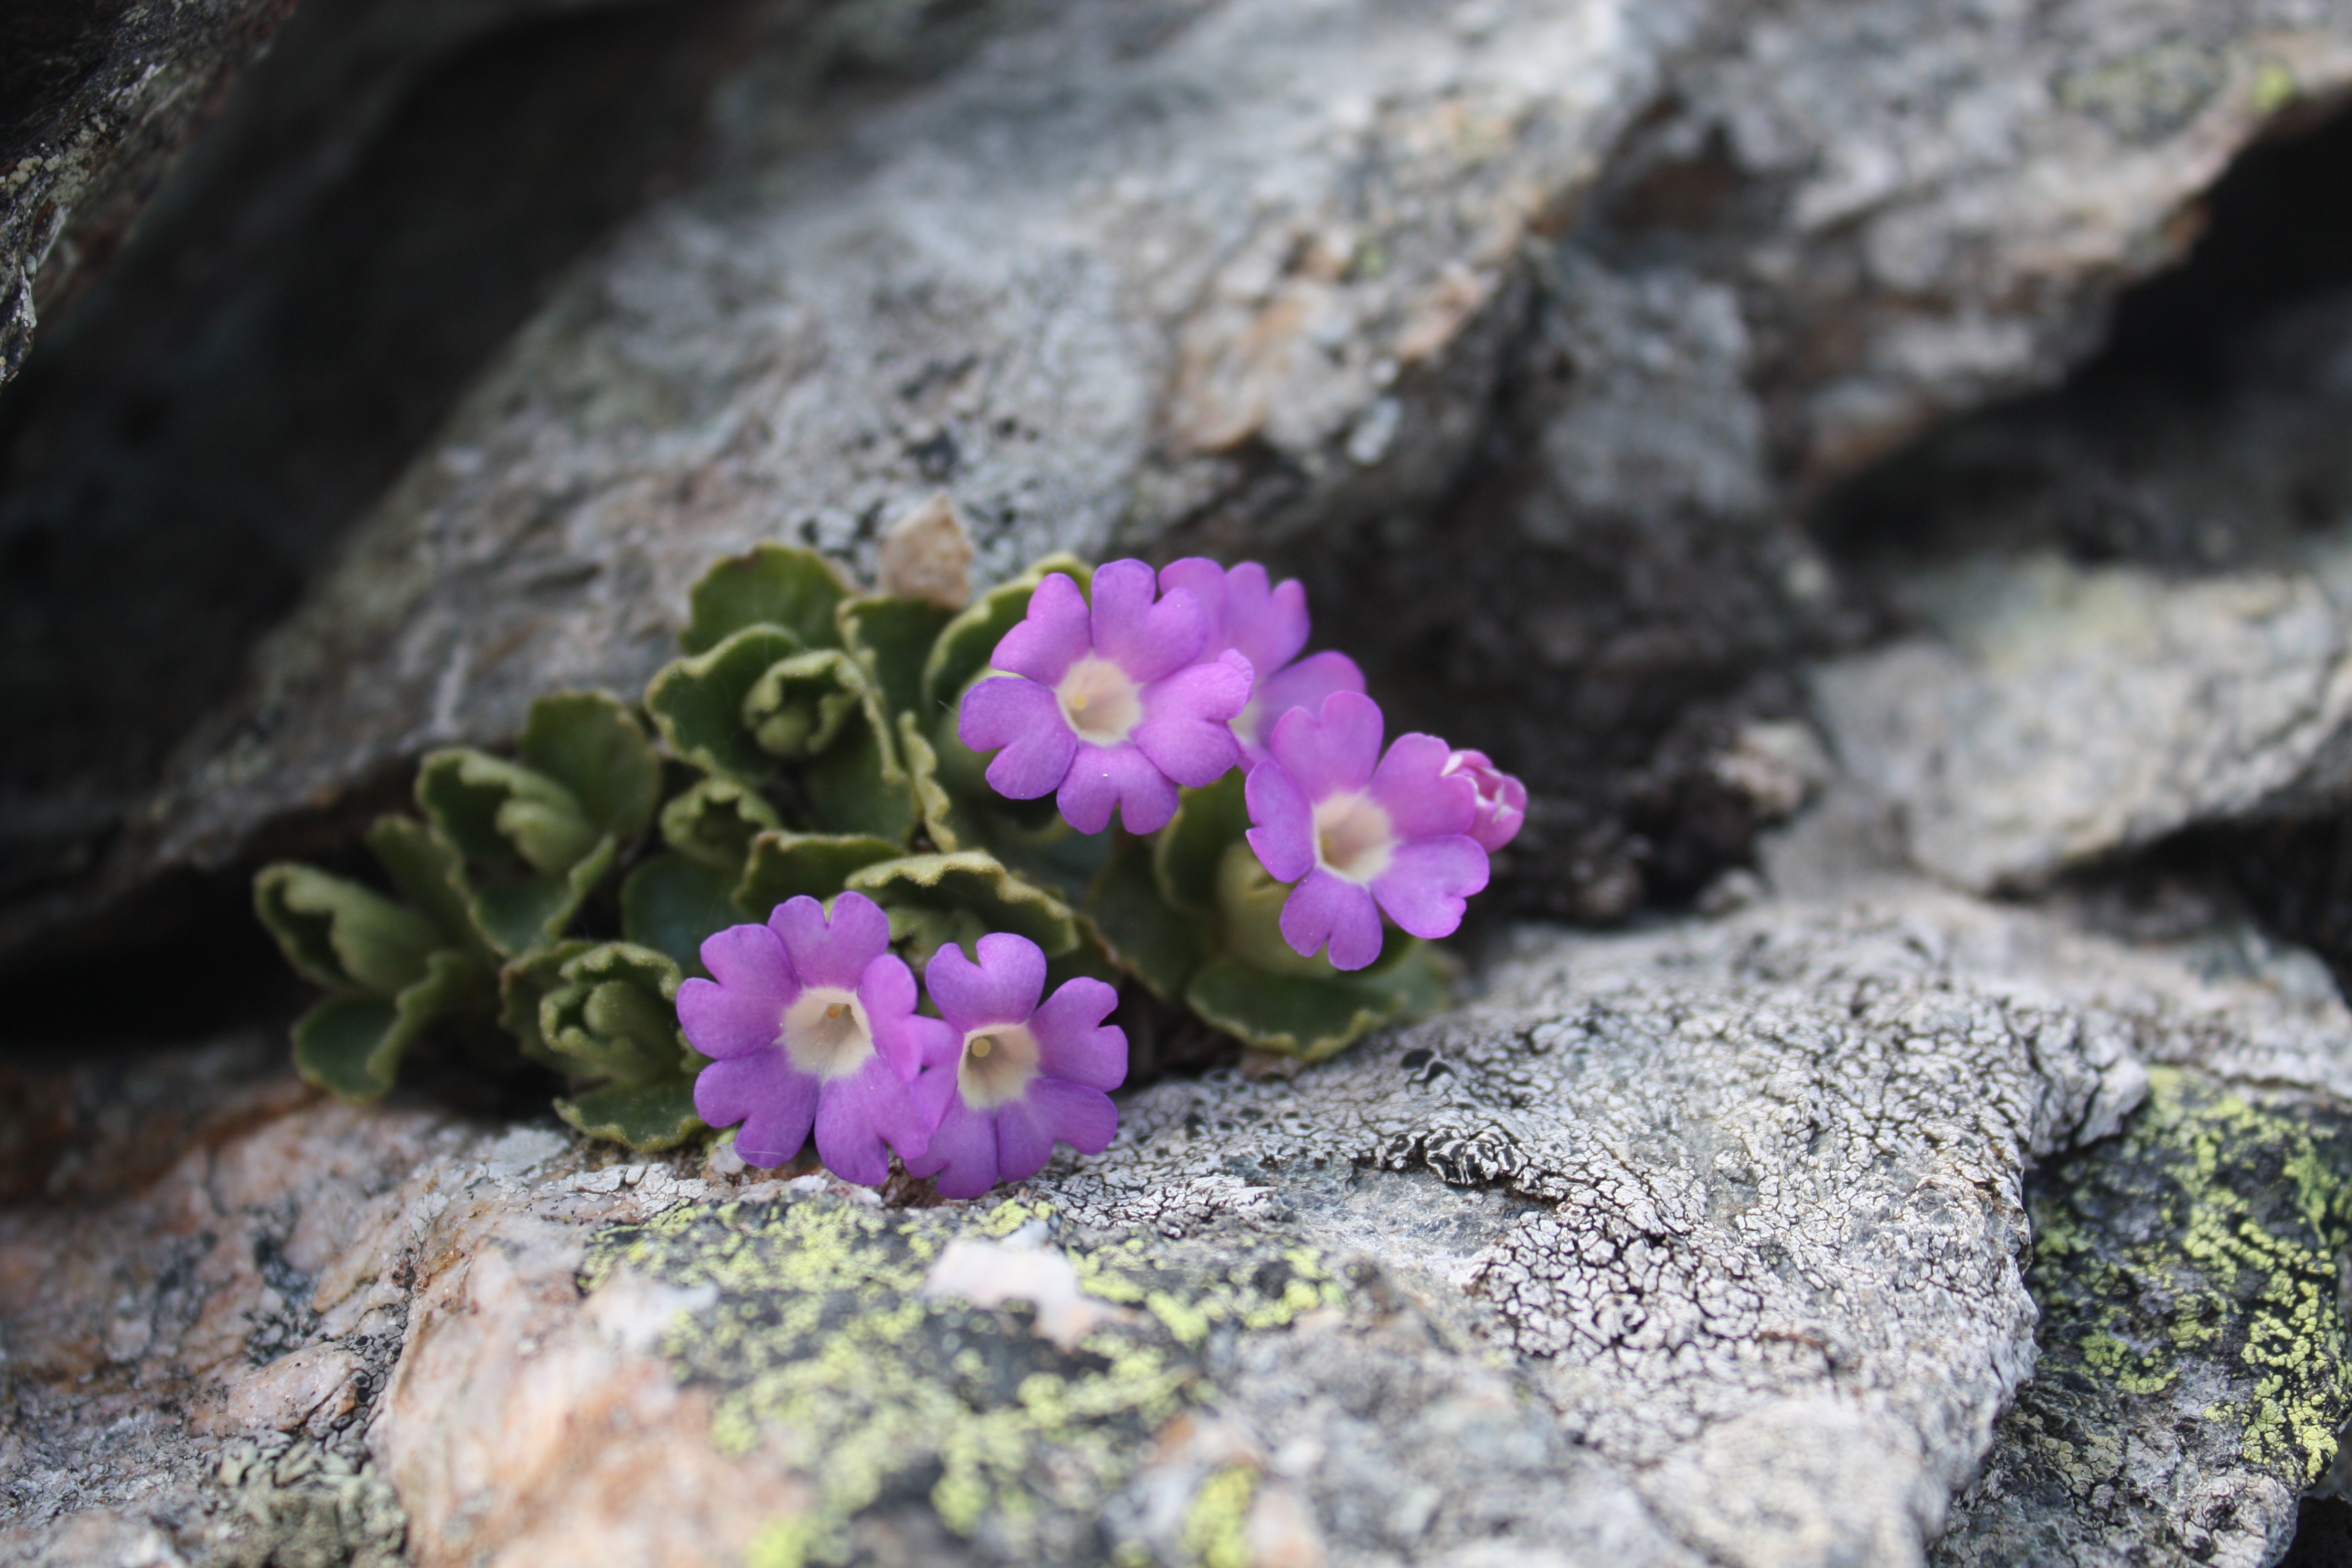
\includegraphics[height = 9.5cm]{fig/Primula_hirsuta_Grand_Chat_longistyle.JPG}
\end{center}
\end{figure}
\thispagestyle{empty}

{\let\thefootnote\relax\footnote{{\noindent Image : \textit{Primula hirsuta}, Florian Boucher~|~Contact:  \href{mailto:maxime.jaunatre@etu.univ-grenoble-alpes.fr}{Mail $^1$}} 
}}
\end{titlepage}

}{
% minipage
\begin{figure}
   \centering
    \begin{minipage}{.75\textwidth}
    \begin{center}
    {\Large Title which is really important and not so much clickbait}
    \end{center}
    %\vspace{\baselineskip}
    %\setlength{\parskip}{\smallskipamount}
    \rule{7em}{.4pt}\par
    %\todo[color = red]{put ellie}
     Maxime Jaunatre $^1$ ~ | Master 2 BEE Grenoble \par 
	\href{mailto:maxime.jaunatre@etu.univ-grenoble-alpes.fr}{Mail $^1$}~| \today \par 
     %\href{mailto:Julia.Julia@etu.univ-grenoble-alpes.fr,maxime.jaunatre@etu.univ-grenoble-alpes.fr}{Mail} | \today
\end{minipage}
\end{figure}

\hrule
}
}
%===================================================================%
%\end{}
%===================================================================%
%%%%%%%%%%%%%%%%%%%%%%%%%%%%%%%%%%%%%%%%%%%%%%%%%%%%%%%%%%%%%%%%%%%%%%
% Abstract
% ignore todo in wordcount !
%TC:macro \todo [0]
%%%%%%%%%%%%%%%%%%%%%%%%%%%%%%%%%%%%%%%%%%%%%%%%%%%%%%%%%%%%%%%%%%%%%%
\ifthenelse{\boolean{title_follow}}{
	\newpage
	\begin{abstract}

	\lipsum[1]
	\imp

	\begin{center}
	\textbf{Abstract}
	\end{center}

	\lipsum[1]
	\imp

	\end{abstract}
	\todo[inline,color=gray]{note that this is an example of abstract in 2 language}
}{
	\textbf{\underline{Abstract :}
	\lipsum[1]
	\imp
	}
	\hrule
}

%%%%%%%%%%%%%%%%%%%%%%%%%%%%%%%%%%%%%%%%%%%%%%%%%%%%%%%%%%%%%%%%%%%%%%
% Table des matières
%%%%%%%%%%%%%%%%%%%%%%%%%%%%%%%%%%%%%%%%%%%%%%%%%%%%%%%%%%%%%%%%%%%%%%
\ifthenelse{\boolean{title_follow}}{
	\newpage
	\tableofcontents
	\thispagestyle{empty}
	\todo[inline,color=gray]{note that this page style is 'empty' and have no page number for example}
}{
}
%%%%%%%%%%%%%%%%%%%%%%%%%%%%%%%%%%%%%%%%%%%%%%%%%%%%%%%%%%%%%%%%%%%%%%
% Todo list
%%%%%%%%%%%%%%%%%%%%%%%%%%%%%%%%%%%%%%%%%%%%%%%%%%%%%%%%%%%%%%%%%%%%%%
\ifthenelse{\boolean{notes}}{
	\ifthenelse{\boolean{title_follow}}{
	\newpage}{}
	\listoftodos
	\hrule\bigskip 
}{}
\todo[inline,color=gray]{note that this todo list will disappear if you set notes on false or comment it}
%%%%%%%%%%%%%%%%%%%%%%%%%%%%%%%%%%%%%%%%%%%%%%%%%%%%%%%%%%%%%%%%%%%%%%
% BODY
\ifthenelse{\boolean{title_follow}}{
	\newpage
}{
}

This document provide all the command I usually use for my reports. Gray notes are here to explain some stuff, while red ones are here to be a last line limit when I wrote my report too close to the deadline and misread colours. I defined a new todonotes juste for this, to help me manage my work. 

\imp[imp command]

\section{Basic command}

Here is some memory about basic latex commands. Like putting some text in \textit{italic} for species names. Or \textbf{bold} for important parts. This is completed with a possibility to highlight with the \hl{hl} command. The colour is defined at the very beginning of the document, but another command allow to change with \hlc[red]{hlc[red]word}. Every colour is possible and you can define them by the xcolor package.

Below is an exemple of a list

\begin{itemize}
  \item Item A.
  \item Item B.
  \begin{enumerate}
  	\item sub part 1
  	\item sub part 2
  \end{enumerate}
  \item Item C
\end{itemize}

\section{To do notes}

To help in long work redaction, the todonotes package is loaded by default, allowing to set inline or marge todonotes \todo[color = gray]{marge}. Authors can be specified and the list of to do is loaded at the beginning of the document. Everything is explain in more detail inside this document \url{http://tug.ctan.org/macros/latex/contrib/todonotes/todonotes.pdf}

\todo[inline, color = gray]{inline}
\todo[inline, author = Gowachin, color = gray]{specifying the author of the todo comment}

% \input{tex/Class.tex}

\section{Maths}

Some packages are also loaded to allow maths equations to be displayed.

\begin{equation}
Y \in B;  B = {a,c,g,t}
\label{eq:11}
\end{equation}

\begin{equation}
\begin{cases}
prey_{t+1} = prey_{t} + prey_{t} \cdot r \cdot (1 - prey_{t} / K ) + int_{pred/prey} \cdot pred_{t} \\
pred_{t+1} = pred_{t} + pred_{t} \cdot r \cdot (1 - pred_{t} / K ) + int_{prey/pred} \cdot prey_{t}
\end{cases}
\label{eq:lotk}
\end{equation}
\textit{with : \textbf{r} the growth rate and \textbf{K} the capacity.} \\

\section{Captions}

Multiple captions are possible, like tables, figures and boxes, as display below. To show all the possibilities, there is \textbf{Lorem ipsum} text around. 

\begin{wrapfigure}{R}{3.10in}
\begin{wordbox}
 \\ \defi{Phylogeny}{Object resuming evolutionary relation between living beings by illustrating distance between them. Mostly represented as a phylogenetic tree.}\\
\defi{Community}{An assemblage of populations from different species, defined by a time and geographic scale restriction. This assemblage can also be represented by interactions between these populations.}\\
\end{wordbox}
%\vspace{-20pt}
\end{wrapfigure}

\lipsum[1-3]

\begin{figure}[h] %{R}{3.00in}
\begin{bluebox}{More complex null model, Pigot \textit{et al.} (2015) \\}

\textbf{Context: }To study the assembly processes of a community, ecologist compare metrics (in this example the Mean Nearest Taxon Distance) with randow draw species in the community. This null model is easily applicable but build assumption issues. For example, these null models don't take into account the historical aspect of community assembly.

\textbf{Results: }Authors found that their null models produce overdispersed community, by just taking into account historical aspect of colonisation and extinction in contrast with just random draw of species. Empirical data shown significantly  overdispersed species in the community but fail to reject this null model. 

Therefore, overdispertion could just arise from historical processes, independent from traits or biotic interactions. This new null model invite us to rethink more precedent result where overdispersion had been found.

%\begin{figure}
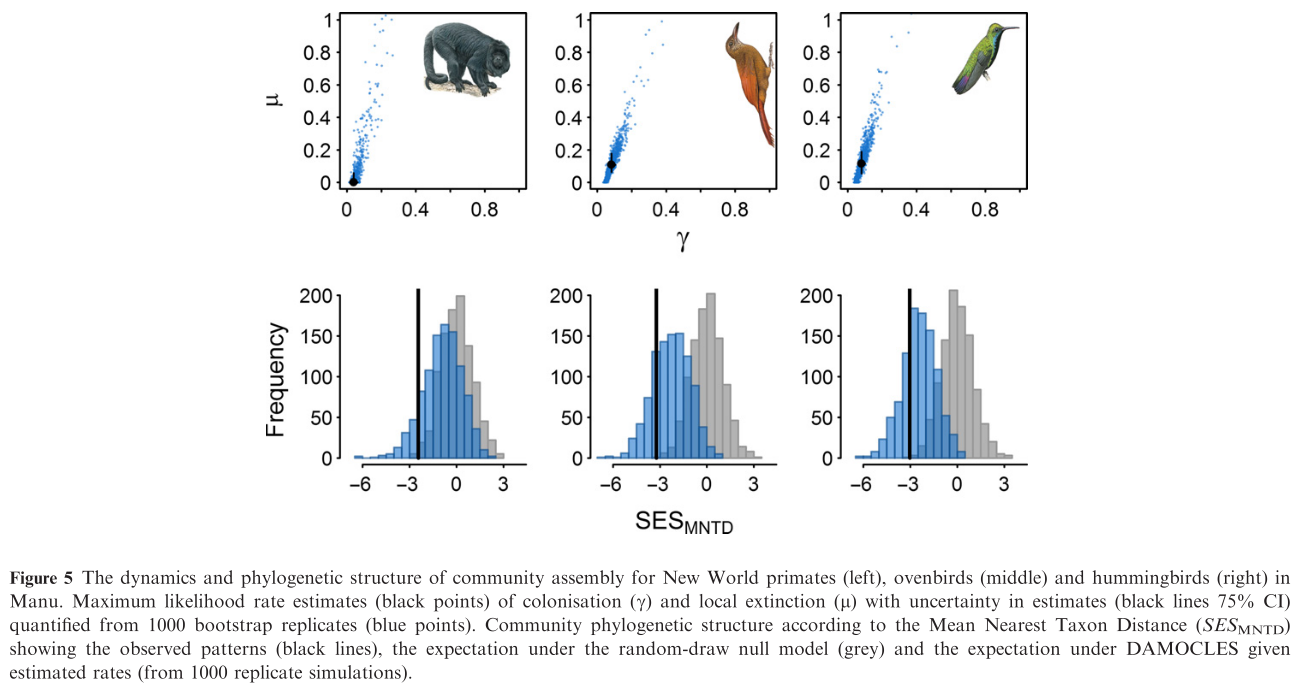
\includegraphics[width=\textwidth]{fig/Pigot2015.png}
%\caption{•}
%\end{figure}
%\vspace{-20pt}
\label{box:Pigot}
\end{bluebox}
\end{figure}

\lipsum[1-3]

\subsection{multicols}

Captions are harder to set in twocolumn environnement, but here is an example.

\begin{multicols}{2} 
\lipsum[1-3] 
\end{multicols}

\section{Import other documents}

\subfile{tex/subpart1}

%%%%%%%%%%%%%%%%%%%%%%%%%%%%%%%%%%%%%%%%%%%%%%%%%%%%%%%%%%%%%%%%%%%%%%
% Références
%%%%%%%%%%%%%%%%%%%%%%%%%%%%%%%%%%%%%%%%%%%%%%%%%%%%%%%%%%%%%%%%%%%%%%
\newpage
\cite{}
\subsection*{Bibliographie}
\imp[change bibliography model]
\ifthenelse{\boolean{bib_basic}}{
	\bibliographystyle{authordate1}
}{
	\bibliographystyle{tree}
	%\bibliographystyle{mee}
}
\bibliography{ICU}

\begin{web}[h]
	\caption{\url{ https://github.com}}
	\label{igp}
\end{web}

%%%%%%%%%%%%%%%%%%%%%%%%%%%%%%%%%%%%%%%%%%%%%%%%%%%%%%%%%%%%%%%%%%%%%%
% Ressources
%%%%%%%%%%%%%%%%%%%%%%%%%%%%%%%%%%%%%%%%%%%%%%%%%%%%%%%%%%%%%%%%%%%%%%
\subsection*{Ressources}

Ce document est disponible en ligne sous format ``.Rnw'', contenant tout le code néccessaire à la reproduction de l'analyse, réalisée avec un script en langage R \citep{RTeam2017}, ainsi que le jeu de données de départ. L'ensemble est situé sur Github : ~\url{https://github.com/gowachin/Template}

%%%%%%%%%%%%%%%%%%%%%%%%%%%%%%%%%%%%%%%%%%%%%%%%%%%%%%%%%%%%%%%%%%%%%%
% Annexes
%%%%%%%%%%%%%%%%%%%%%%%%%%%%%%%%%%%%%%%%%%%%%%%%%%%%%%%%%%%%%%%%%%%%%%
\newpage
 \begin{landscape}
 \begin{annexe}
 	\centering
 \rowcolors{2}{white}{gray!25}
 \resizebox{27cm}{!}{%
 	\begin{tabular}{cccccccccccc}
 	\toprule
 Species &Locality &Code &Morph &Collector &Date &Longitude &Latitude &Altitude&Reads raw &Reads trimmed &Voucher \\
 	\midrule
 P. apennina* &Sella del Marmagna, Italy &AMB &Short-styled &F. Boucher/L. Gallien &30/05/14 & 10.00575 & 44.3978 &1610&6885928&6486849&Photo \\
 P. apennina &Monte Marmagna, Italy &AML &Long-styled &F. Boucher/L. Gallien &30/05/14 & 9.99731 & 44.39672 &1825&1856867&1663377&Photo \\
 P. apennina &Monte Orsaro, Italy &AOL &Long-styled &F. Boucher/L. Gallien &30/05/14 & 9.99666 & 44.39883 &1818&3494081&3230296&Photo \\
 P. cottia &Below locus classicus, Italy &CS1 & NA &F. Boucher &23/07/14 & 7.0716 & 44.9271 &1159&5127416&4814386&Photo \\
  P. apennina* &Sella del Marmagna, Italy &AMB &Short-styled &F. Boucher/L. Gallien &30/05/14 & 10.00575 & 44.3978 &1610&6885928&6486849&Photo \\
 P. apennina &Monte Marmagna, Italy &AML &Long-styled &F. Boucher/L. Gallien &30/05/14 & 9.99731 & 44.39672 &1825&1856867&1663377&Photo \\
 P. apennina &Monte Orsaro, Italy &AOL &Long-styled &F. Boucher/L. Gallien &30/05/14 & 9.99666 & 44.39883 &1818&3494081&3230296&Photo \\
 P. cottia &Below locus classicus, Italy &CS1 & NA &F. Boucher &23/07/14 & 7.0716 & 44.9271 &1159&5127416&4814386&Photo \\
 	\bottomrule
 	\end{tabular}}
 	\caption{\textbf{Exemple d'annexe}}
 	\label{table_ind}
 \end{annexe}
 \end{landscape}

%%%%%%%%%%%%%%%%%%%%%%%%%%%%%%%%%%%%%%%%%%%%%%%%%%%%%%%%%%%%%%%%%%%%%%
% word count
\ifthenelse{\boolean{terminal}}{
	\newpage
	\imp[Remove word counts]
	\ifthenelse{\boolean{counter}}{
		\subsubsection*{Counts of words}
		\wordcount
	}{}
}{}

\end{document}


